
\documentclass[a4paper,class=article,border=0pt,tikz]{standalone}
%\documentclass[class=minimal,border=0pt]{standalone}
%\documentclass{article}
%\usepackage[a4paper,margin=0in,landscape]{geometry}
%\usepackage{fullpage}
%\pagestyle{empty}
\usepackage{xcolor}

%195, 252, 186 = #C3FCBA
\definecolor{infieldCmyk}{cmyk}{0.23,0.00,0.26,1.00}
\definecolor{infieldRgb}{RGB}{195,252,186}
%238, 226, 222 = #EEE2DE 
\definecolor{dirtRgb}{RGB}{238,226,222}
\definecolor{dirtCmyk}{cmyk}{0.00,0.05,0.07,0.07}
%234, 254, 232 = #EAFEE8
\definecolor{backgroundRgb}{RGB}{234,254,232}
\definecolor{backgroundCmyk}{cmyk}{0.08,0.00,0.09,0.00}


%\definecolor{infield}{RGB}{185,110,85}

\usepackage{tikz}
\usepackage{xfrac}

\tikzset{
  atbat/.pic={
  code={\tikzset{scale=.25}
  
\draw[draw=black,very thick,fill=backgroundRgb] (0,0) rectangle ++(8,6);

%balls
\draw[draw=black,thick,fill=white] (0,3) rectangle ++(1,1);
\draw[draw=black,thick,fill=white] (0,4) rectangle ++(1,1);
\draw[draw=black,thick,fill=white] (0,5) rectangle ++(1,1);
%fouls
\draw[draw=black,thick,fill=white] (1,3) rectangle ++(1,1);
\draw[step=.5cm,black] (1,3) grid ++(1,1);

%strikes
\draw[draw=black,thick,fill=white] (1,4) rectangle ++(1,1);
\draw[draw=black,thick,fill=white] (1,5) rectangle ++(1,1);

%diamond
\begin{scope}[shift={(5,.25)},rotate=45,scale=1.25]

%\draw[fill=yellow!30] (0,0) -- (3.25,0) arc[start angle=0, end angle=90,radius=3.5cm] -- (0,0);
\draw[draw=black,very thin,fill=dirtRgb] (0,0) -- (3.25,0) .. controls (3.5,3.5) .. (0,3.25) -- (0,0);

%diamond
\draw[draw=black,thick,dotted,fill=infieldRgb] (0,0) rectangle ++(2.5,2.5);
%home:
%\draw[draw=black,thick] (0,0) rectangle ++(.5,.5);

%3rd
\draw[draw=black,thin,fill=white] (0,2.5) rectangle ++(.5,-.5);
%2nd
\draw[draw=black,thin,fill=white] (2.5,0) rectangle ++(-.5,.5);
%1st 
\draw[draw=black,thin,fill=white] (2.5,2.5) rectangle ++(-.5,-.5);

\end{scope}


  }}
}

\tikzset{
  row/.pic={
  code={\tikzset{scale=1}
\draw[draw=black,thick] (0,0) rectangle ++(.5,1.5);
\draw[draw=black,thick] (.5,0) rectangle ++(2.5,1.5);
\draw[draw=black,thick] (3,0) rectangle ++(.5,1.5);
\draw[draw=black,thick] (3.5,0) rectangle ++(.5,1.5);
\draw[thin] (0,.75) -- (4,.75);
\path (4,0) pic {atbat};
\path (6,0) pic {atbat};
\path (8,0) pic {atbat};
\path (10,0) pic {atbat};
\path (12,0) pic {atbat};
\path (14,0) pic {atbat};
\path (16,0) pic {atbat};
\path (18,0) pic {atbat};
\path (20,0) pic {atbat};
\path (22,0) pic {atbat};
\path (24,0) pic {atbat};
%\draw (26,0) rectangle ++(2,1);

  }}
}

\tikzset{
  grid/.pic={
  code={\tikzset{scale=1}

\path (0,1.5) pic {row};
\path (0,3.0) pic {row};
\path (0,4.5) pic {row};
\path (0,6.0) pic {row};
\path (0,7.5) pic {row};
\path (0,9.0) pic {row};
\path (0,10.5) pic {row};
\path (0,12.0) pic {row};
\path (0,13.5) pic {row};

%header
\draw[draw=black,thick] (0,15) rectangle ++(.5,0.5);
\node (hash) at (.25,15.25) {\#};
\draw[draw=black,thick] (0.5,15) rectangle ++(2.5,0.5);
\node (player) at (1.5,15.25) {\textsc{Player}};

\draw[draw=black,thick] (3,15) rectangle ++(0.5,0.5);
\node (lr) at (3.25,15.25) {$\sfrac{\textsc{l}}{\textsc{r}}$};

\draw[draw=black,thick] (3.5,15) rectangle ++(0.5,0.5);
\node (pos) at (3.75,15.25) { \textsc{p} };

\draw[draw=black,thick] (4,15) rectangle ++(2,0.5);
\node (one) at (5,15.25) { \textbf{1} };
\draw[draw=black,thick] (6,15) rectangle ++(2,0.5);
\node (one) at (7,15.25) { \textbf{2} };
\draw[draw=black,thick] (8,15) rectangle ++(2,0.5);
\node (one) at (9,15.25) { \textbf{3} };
\draw[draw=black,thick] (10,15) rectangle ++(2,0.5);
\node (one) at (11,15.25) { \textbf{4} };
\draw[draw=black,thick] (12,15) rectangle ++(2,0.5);
\node (one) at (13,15.25) { \textbf{5} };
\draw[draw=black,thick] (14,15) rectangle ++(2,0.5);
\node (one) at (15,15.25) { \textbf{6} };
\draw[draw=black,thick] (16,15) rectangle ++(2,0.5);
\node (one) at (17,15.25) { \textbf{7} };
\draw[draw=black,thick] (18,15) rectangle ++(2,0.5);
\node (one) at (19,15.25) { \textbf{8} };
\draw[draw=black,thick] (20,15) rectangle ++(2,0.5);
\node (one) at (21,15.25) { \textbf{9} };
\draw[draw=black,thick] (22,15) rectangle ++(2,0.5);
\node (one) at (23,15.25) { \textbf{10} };
\draw[draw=black,thick] (24,15) rectangle ++(2,0.5);
\node (one) at (25,15.25) { \textbf{11} };

  }}
}


\tikzset{
  boxscore/.pic={
  code={\tikzset{scale=1}
  
\draw[step=1cm,black] (3,0) grid ++(14,2);
\draw[black] (0,1) -- ++(3,0);
\draw[draw=black,very thick] (0,0) rectangle ++(17,2);
\node[above] (teams) at (1.5,2) {\textsc{Teams}};
\foreach \i in {1,2,...,11}{
    \node[above] (inning\i) at (2.5 + \i,2) {\textsc{$\i$}};
}
\draw[very thick] (3,0) -- ++(0,2);
\node[above] (runs) at (14.5,2) {\textsc{r}};
\draw[very thick] (14,0) -- ++(0,2);
\node[above] (hits) at (15.5,2) {\textsc{h}};
\draw[very thick] (15,0) -- ++(0,2);
\node[above] (errs) at (16.5,2) {\textsc{e}};
\draw[very thick] (16,0) -- ++(0,2);

  }}
}



\begin{document}

%at bat: 1.5cm tall, split in 2
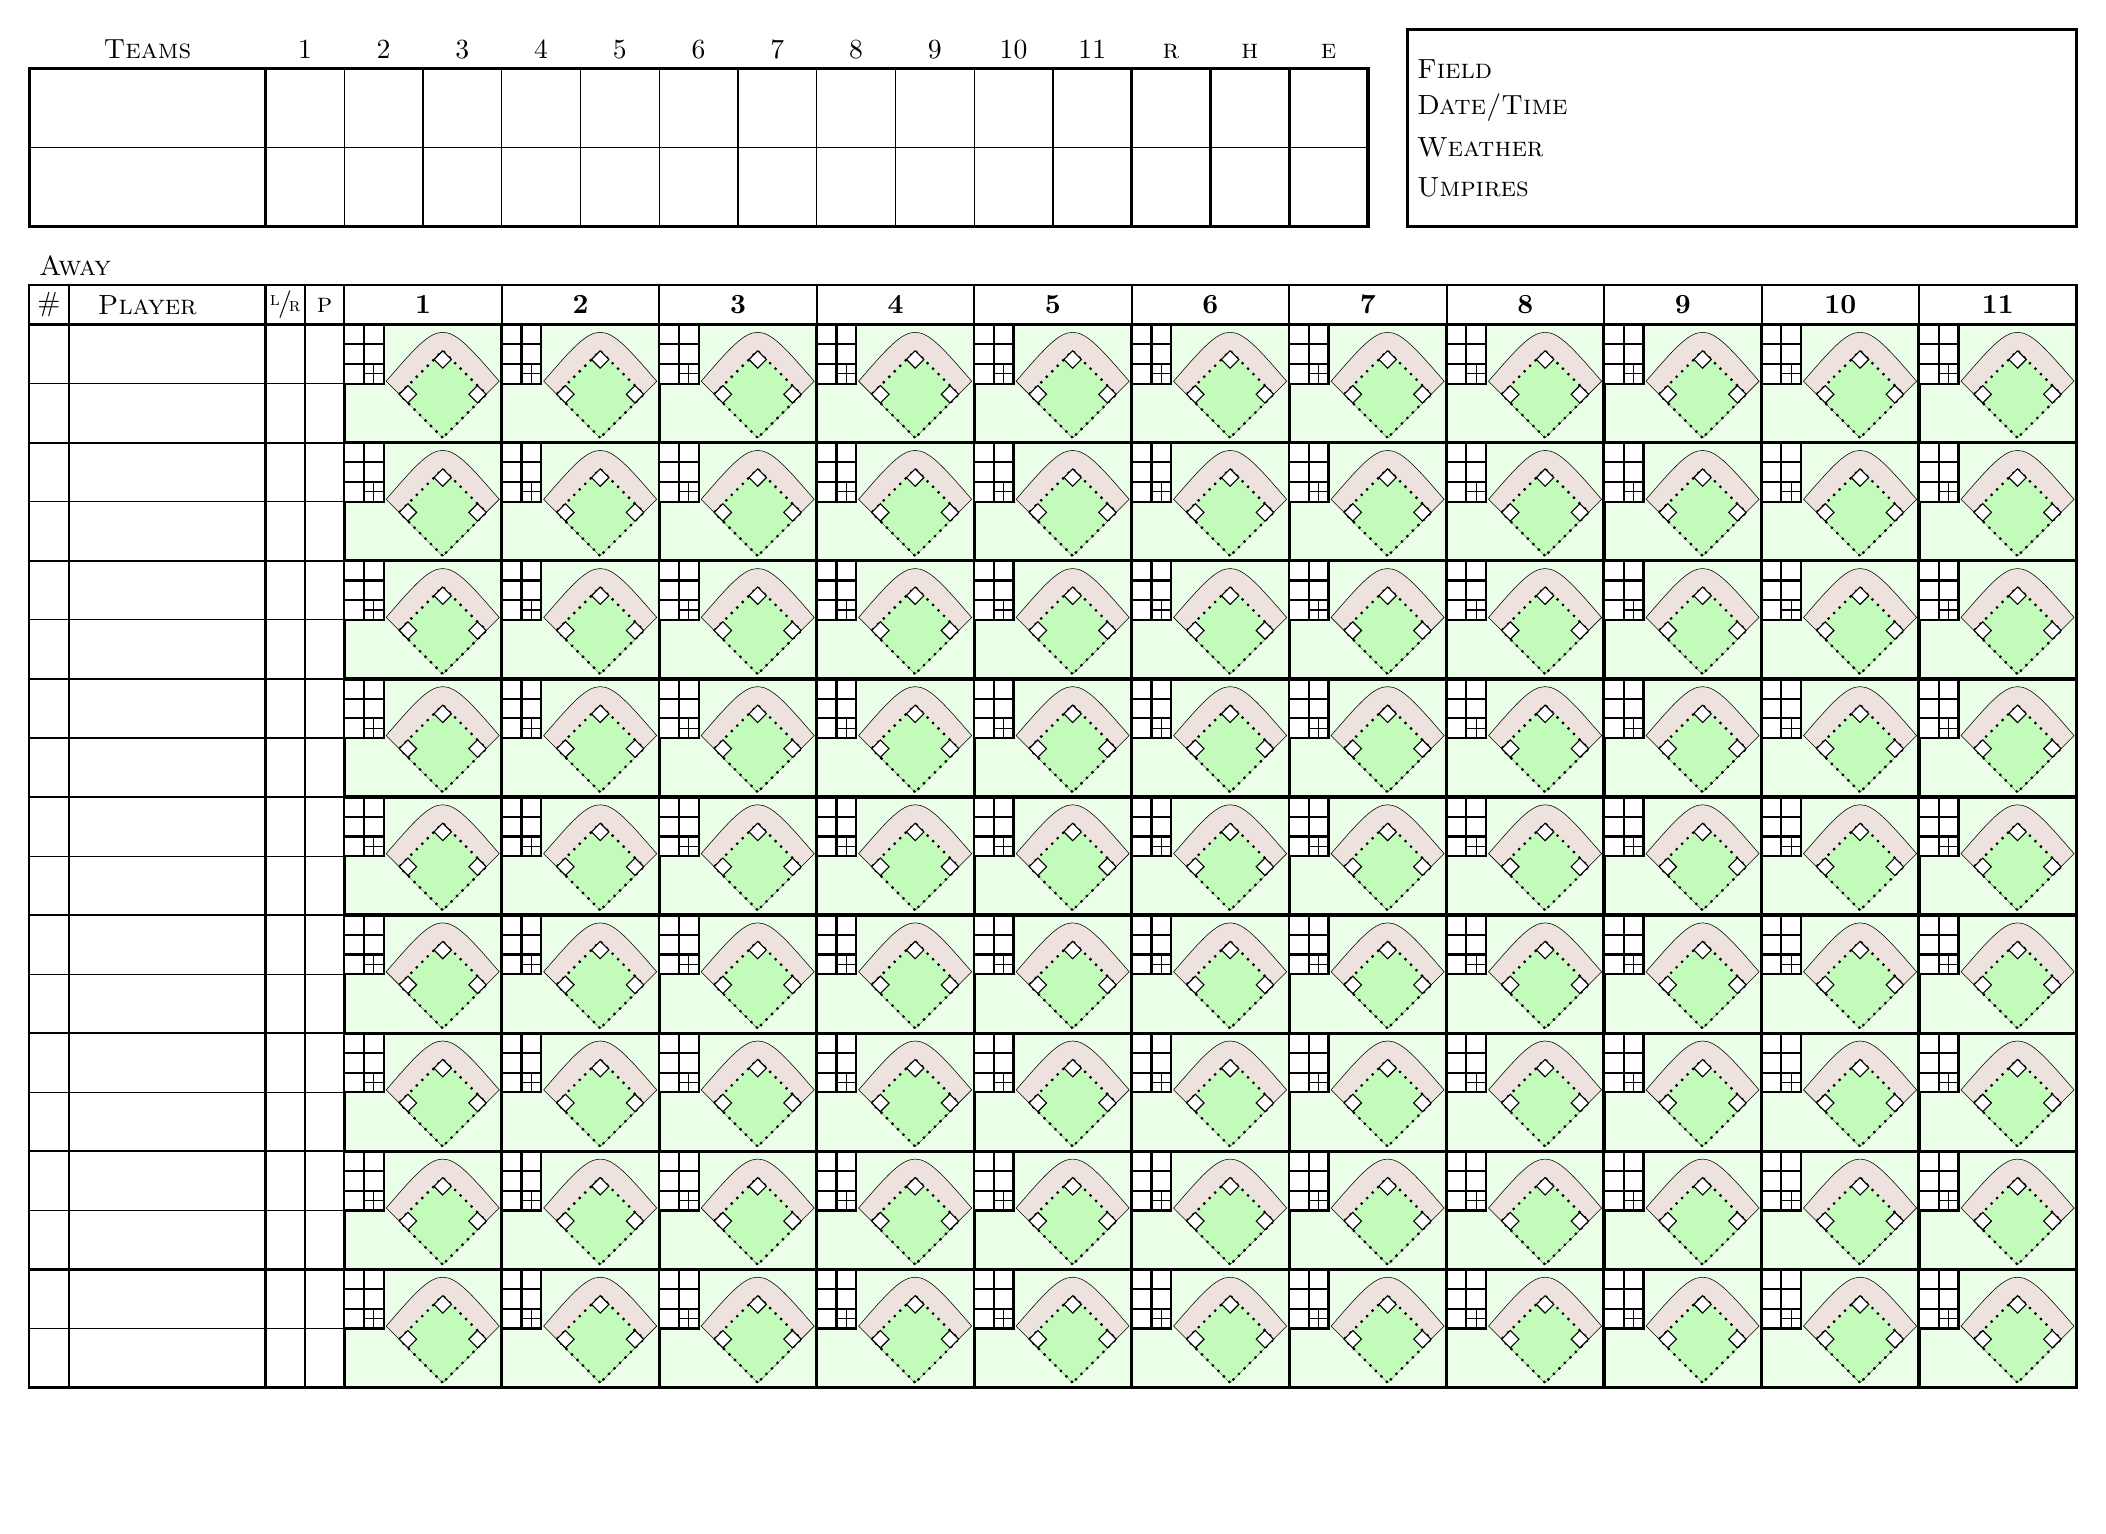
\begin{tikzpicture}

%\draw[step=1cm,gray,very thin] (0,0) grid (28,21);

\path (1,.75) pic {grid};
\node[right] (away) at (1,16.5) {\textsc{Away}};

\path (1,17) pic {boxscore};


\begin{scope}[shift={(18.5,17)},rotate=0,scale=1]

\draw[draw=black,very thick] (0,0) rectangle ++(8.5,2.5);
\node[right] (field) at (0,2) {\textsc{Field}};
\node[right] (date) at (0,1.5) {\textsc{Date/Time}};
\node[right] (weather) at (0,1) {\textsc{Weather}};
\node[right] (umpires) at (0,.5) {\textsc{Umpires}};


\end{scope}



\end{tikzpicture}


%at bat: 1.5cm tall, split in 2
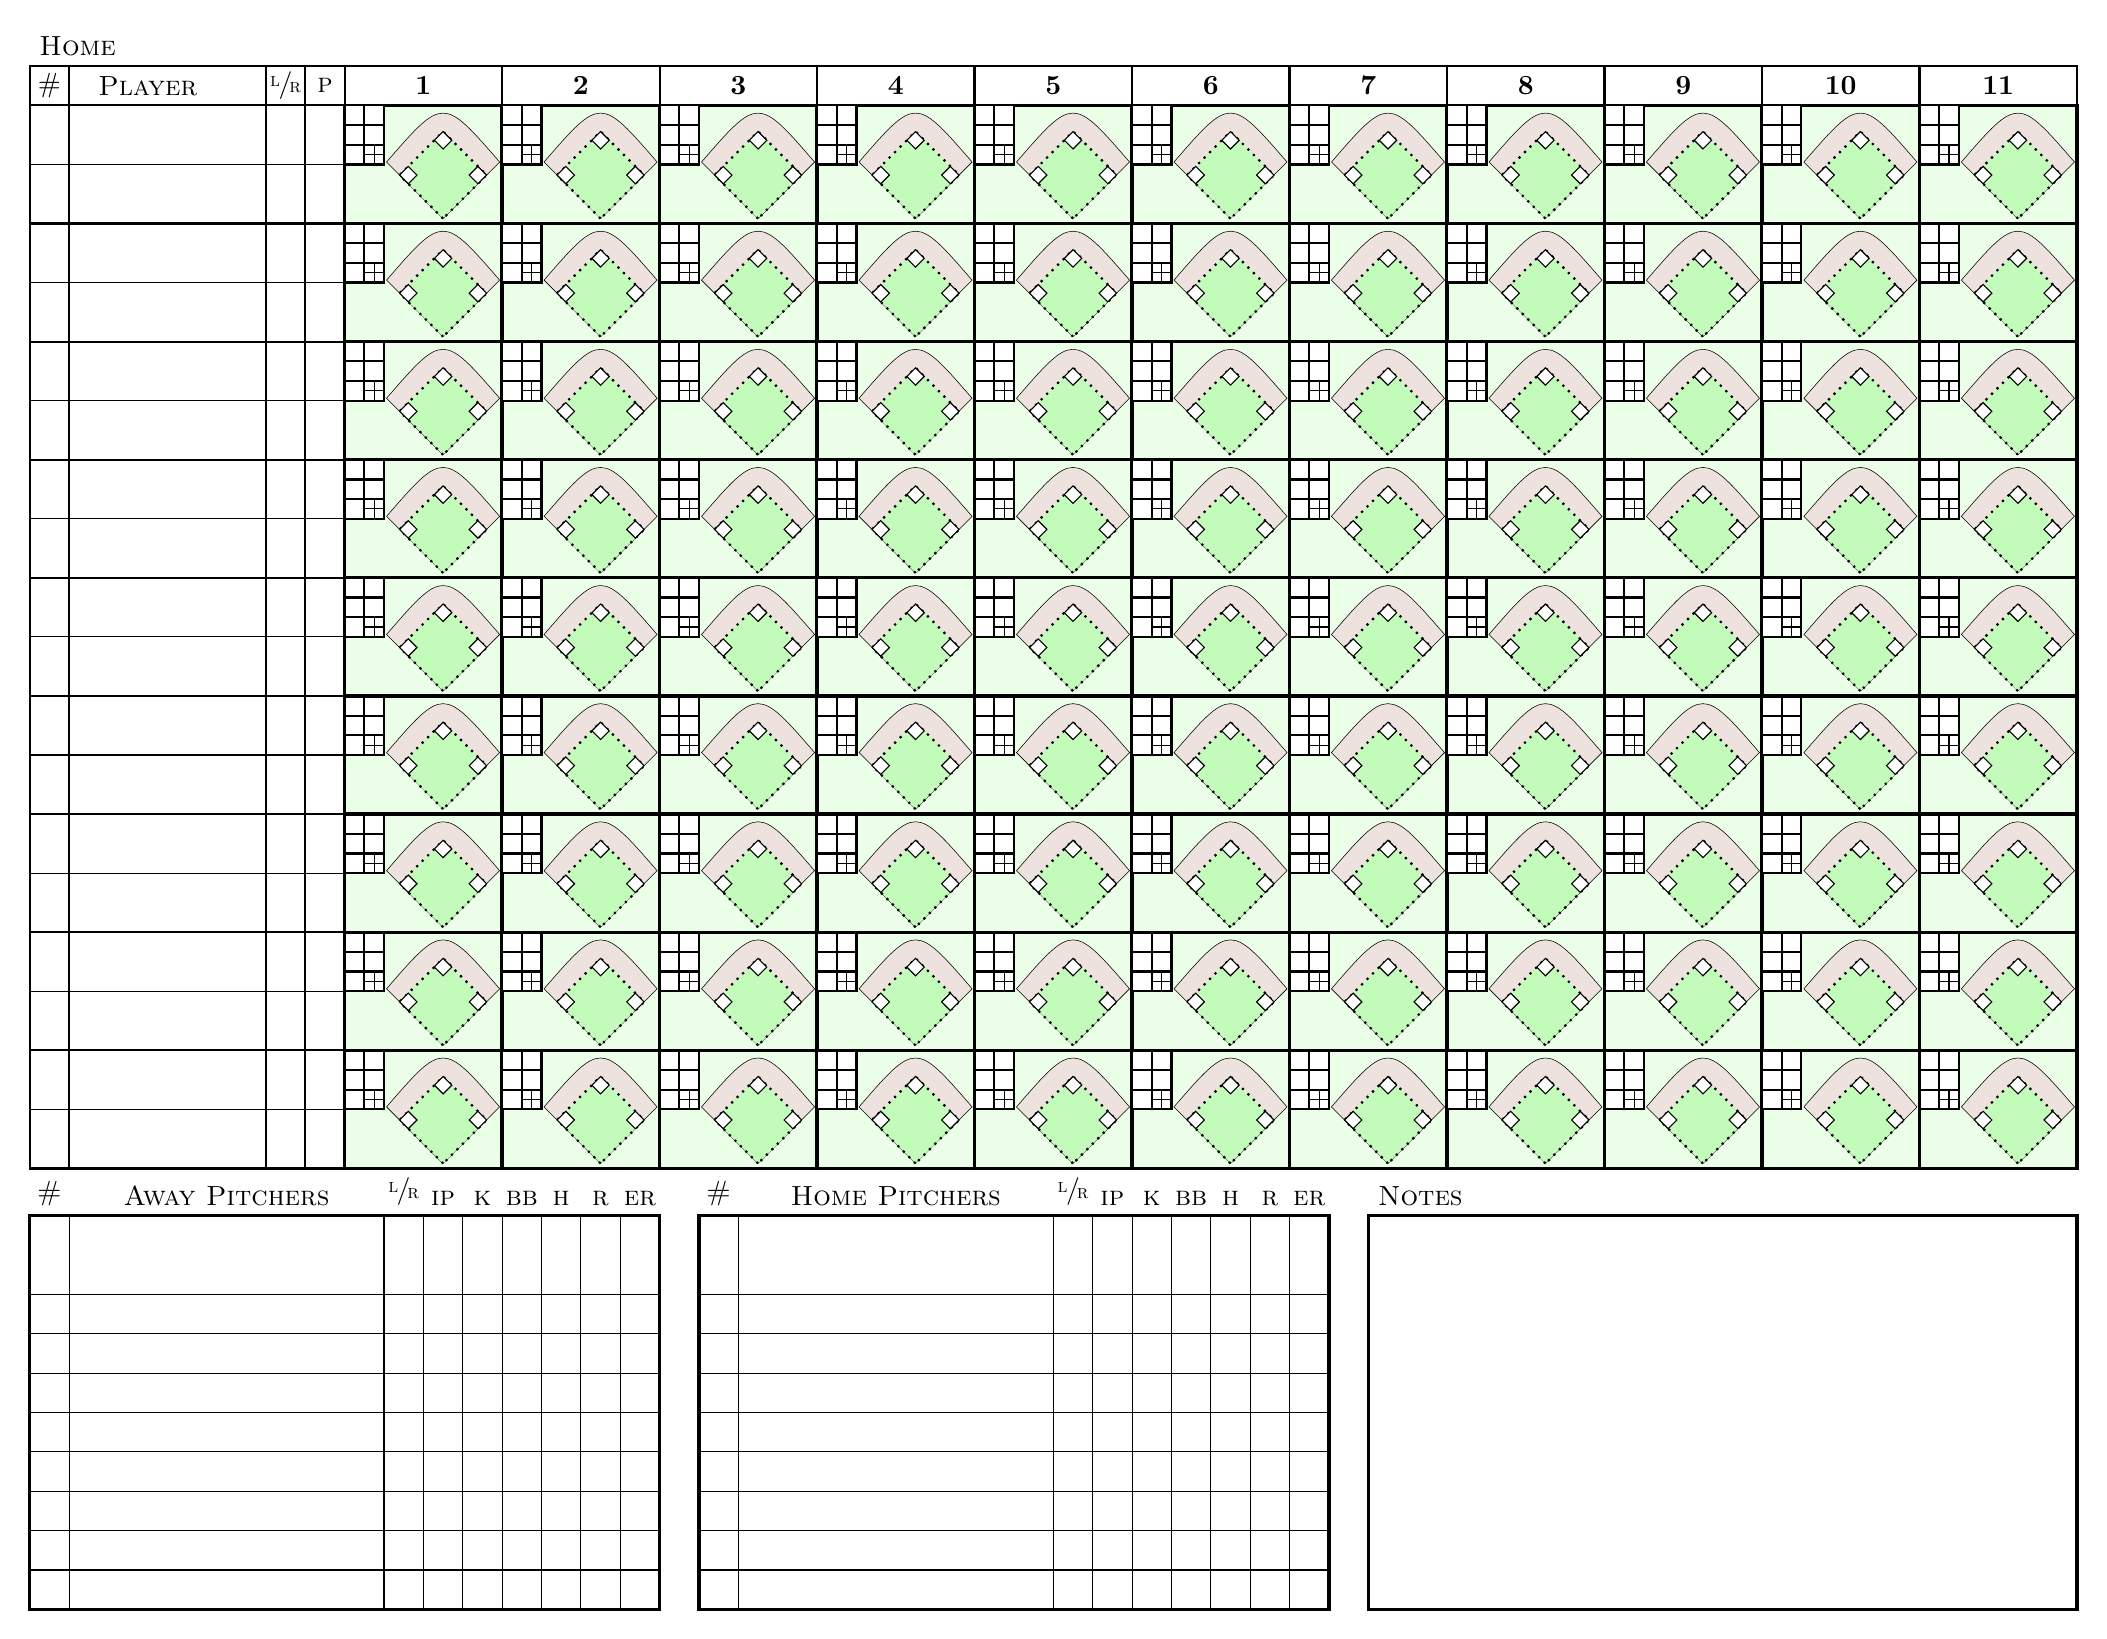
\begin{tikzpicture}[rotate=0,transform shape]

%\draw[step=1cm,gray,very thin] (0,0) grid (28,21);

\path (1,4.5) pic {grid};
\node[right] (home) at (1,20.25) {\textsc{Home}};

%pitcher box
\begin{scope}[shift={(1,1.4)},rotate=0,scale=1]

\draw[draw=black,very thick] (0,-1) rectangle ++(8,5);
%1cm for starting pitcher + notes
\draw[draw=black] (0,4.0) -- ++(8,0);
%.5cm for each subsequent
\draw[draw=black] (0,3.0) -- ++(8,0);
\draw[draw=black] (0,2.5) -- ++(8,0);
\draw[draw=black] (0,2.0) -- ++(8,0);
\draw[draw=black] (0,1.5) -- ++(8,0);
\draw[draw=black] (0,1.0) -- ++(8,0);
\draw[draw=black] (0,0.5) -- ++(8,0);
\draw[draw=black] (0,0.0) -- ++(8,0);
\draw[draw=black] (0,-0.5) -- ++(8,0);
\draw[draw=black] (0,-1) -- ++(8,0);

\draw[draw=black] (.5,-1) -- ++(0,5);
\node[above] (num) at (.25,4) {\textsc{\#}};
\node[above] (pitcher) at (2.5,4) {\textsc{Away Pitchers}};

\node[above] (lr) at (4.75,4) {$\sfrac{\textsc{l}}{\textsc{r}}$};
\draw[draw=black] (4.5,-1) -- ++(0,5);
\node[above] (ip) at (5.25,4) {\textsc{ip}};
\draw[draw=black] (5.0,-1) -- ++(0,5);
\node[above] (k) at (5.75,4) {\textsc{k}};
\draw[draw=black] (5.5,-1) -- ++(0,5);
\node[above] (bb) at (6.25,4) {\textsc{bb}};
\draw[draw=black] (6.0,-1) -- ++(0,5);
\node[above] (hits) at (6.75,4) {\textsc{h}};
\draw[draw=black] (6.5,-1) -- ++(0,5);
\node[above] (r) at (7.25,4) {\textsc{r}};
\draw[draw=black] (7.0,-1) -- ++(0,5);
\node[above] (ER) at (7.75,4) {\textsc{er}};
\draw[draw=black] (7.5,-1) -- ++(0,5);

\end{scope}

%pitcher box
\begin{scope}[shift={(9.5,1.4)},rotate=0,scale=1]

\draw[draw=black,very thick] (0,-1) rectangle ++(8,5);
%1cm for starting pitcher + notes
\draw[draw=black] (0,4.0) -- ++(8,0);
%.5cm for each subsequent
\draw[draw=black] (0,3.0) -- ++(8,0);
\draw[draw=black] (0,2.5) -- ++(8,0);
\draw[draw=black] (0,2.0) -- ++(8,0);
\draw[draw=black] (0,1.5) -- ++(8,0);
\draw[draw=black] (0,1.0) -- ++(8,0);
\draw[draw=black] (0,0.5) -- ++(8,0);
\draw[draw=black] (0,0.0) -- ++(8,0);
\draw[draw=black] (0,-0.5) -- ++(8,0);
\draw[draw=black] (0,-1) -- ++(8,0);


\draw[draw=black] (.5,-1) -- ++(0,5);
\node[above] (num) at (.25,4) {\textsc{\#}};
\node[above] (pitcher) at (2.5,4) {\textsc{Home Pitchers}};

\node[above] (lr) at (4.75,4) {$\sfrac{\textsc{l}}{\textsc{r}}$};
\draw[draw=black] (4.5,-1) -- ++(0,5);
\node[above] (ip) at (5.25,4) {\textsc{ip}};
\draw[draw=black] (5.0,-1) -- ++(0,5);
\node[above] (k) at (5.75,4) {\textsc{k}};
\draw[draw=black] (5.5,-1) -- ++(0,5);
\node[above] (bb) at (6.25,4) {\textsc{bb}};
\draw[draw=black] (6.0,-1) -- ++(0,5);
\node[above] (hits) at (6.75,4) {\textsc{h}};
\draw[draw=black] (6.5,-1) -- ++(0,5);
\node[above] (r) at (7.25,4) {\textsc{r}};
\draw[draw=black] (7.0,-1) -- ++(0,5);
\node[above] (ER) at (7.75,4) {\textsc{er}};
\draw[draw=black] (7.5,-1) -- ++(0,5);

\end{scope}

%notes
\begin{scope}[shift={(18,1.4)},rotate=0,scale=1]

\draw[draw=black,very thick] (0,-1) rectangle ++(9,5);
\node[above right] (notes) at (0,4) {\textsc{Notes}};

\end{scope}



\end{tikzpicture}


\end{document}